\chapter{Vegetatieve ontwikkeling van planten: meristemen en groei}\label{ch:b2:plant-meristems}

Een eik die een zaailing was toen de kathedraal werd gebouwd, legt nog elk
jaar een ring \omterm{def:b2:plant-meristems:wood}{hout} aan, opent nog elk voorjaar nieuwe bladeren, duwt nog
nieuwe worteltoppen door de grond. Geen enkel dier doet dat; een paard
houdt op vierjarige leeftijd op met groeien. Het verschil is dat een plant
aan de top van elke scheut en elke wortel, en in een dunne cilinder in elke
stam, kleine populaties embryonale cellen behoudt --- de \emph{meristemen}
--- die nooit ophouden met delen en die het lichaam van de plant zo lang
als ze leeft naar buiten en naar boven uitbouwen. Dit hoofdstuk bekijkt hoe
de twee apicale meristemen georganiseerd en gestuurd zijn, hoe een
plantencel groeit, hoe hormonen de vorm van een scheut bepalen, en hoe een
stam dikker wordt.

\section{Meristemen}

\begin{definition}[Meristemen en de twee soorten groei]\label{def:b2:plant-meristems:meristem}
\index{meristeem}\index{apicaal scheutmeristeem}\index{apicaal wortelmeristeem}\index{cambium}
Een \emph{meristeem} is een populatie kleine, ongedifferentieerde, delende
cellen die het hele leven van de plant blijft bestaan en waaruit al haar
weefsels voortkomen. Het \emph{apicaal scheutmeristeem} (SAM) aan de top
van elke scheut maakt bladeren, stengel en, in het seizoen, \omterm{def:b2:angiosperm-reproduction:flower}{bloemen}; het
\emph{apicaal wortelmeristeem} (RAM) achter elke worteltop maakt de wortel;
samen drijven ze de \emph{primaire groei} aan, het langer worden van de
plant. De \emph{laterale meristemen} --- het \emph{\omterm{def:b2:plant-meristems:wood}{vaatcambium}} en het
\emph{kurkcambium}, dunne cilinders in stengels en wortels --- drijven de
\emph{secundaire groei} aan, de verdikking die \omterm{def:b2:plant-meristems:wood}{hout} en schors maakt.
Plantengroei is daardoor \emph{onbegrensd}: de meristemen kunnen
onbeperkt doorgaan, en de plant is een modulair organisme dat de eenheid
blad--knoop--internodium--knop herhaalt zolang de omstandigheden het
toelaten. Elke okselknop is een slapend SAM, zodat een plant duizenden
reservegroeipunten meedraagt.
\end{definition}

\begin{proposition}[De scheuttop]\label{prop:b2:plant-meristems:sam}
\index{fyllotaxis}\index{bladprimordium}\index{plastochron}
Het SAM is een koepel van een tiende millimeter doorsnede, met enkele
honderden cellen. De buitenste een of twee lagen (de \emph{tunica}) delen
zich alleen in het vlak van het oppervlak en vormen de epidermis; de massa
eronder (het \emph{corpus}) deelt zich in alle vlakken. Op de top voedt een
\emph{centrale zone} van langzaam delende stamcellen een \emph{perifere
zone} van sneller delende cellen, waar \emph{bladprimordia} als bulten
ontstaan met regelmatige tussenpozen in de tijd (het \emph{plastochron},
uren tot dagen) en onder regelmatige hoeken rond de koepel (de
\emph{fyllotaxis}: tegenoverstaand, kransstandig, of spiraalsgewijs onder de
gulden hoek van \qty{137.5}{\degree}, die elk nieuw blad in de grootste
opening tussen de andere plaatst). Daaronder maakt een \emph{ribzone} het
merg en verlengt ze de stengel. Een primordium ontstaat waar het hormoon
auxine zich in de oppervlaktelaag ophoopt, en terwijl het groeit, onttrekt
het auxine aan zijn omgeving, waardoor het volgende primordium er zo ver
mogelijk vandaan ontstaat: het patroon organiseert zichzelf.
\end{proposition}

\begin{omfigure}
\begin{tikzpicture}[every node/.style={font=\scriptsize}]
  % dome
  \draw[thick, fill=omExo!12] (-2.2,0) .. controls (-2.2,1.6) and (-0.8,2.6) .. (0,2.6) .. controls (0.8,2.6) and (2.2,1.6) .. (2.2,0) -- (2.2,-1.4) -- (-2.2,-1.4) -- cycle;
  % tunica layers
  \draw[thick, omDef] (-2.2,0) .. controls (-2.2,1.5) and (-0.8,2.45) .. (0,2.45) .. controls (0.8,2.45) and (2.2,1.5) .. (2.2,0);
  \draw[thick, omDef] (-2.05,0) .. controls (-2.05,1.35) and (-0.75,2.3) .. (0,2.3) .. controls (0.75,2.3) and (2.05,1.35) .. (2.05,0);
  % zones
  \draw[thick, dashed, omThm, fill=omThm!15] (0,1.75) ellipse (0.6 and 0.55);
  \draw[thick, dashed, omProp] (0,0.9) ellipse (1.6 and 1.35);
  \draw[thick, dashed, omExo!70!black] (-0.9,-0.9) rectangle (0.9,-0.1);
  % primordia
  \draw[thick, fill=omExo!40] (-2.2,0.4) .. controls (-2.5,1.4) and (-1.6,1.9) .. (-1.55,1.3) .. controls (-1.5,0.9) and (-1.9,0.6) .. (-2.2,0.4);
  \draw[thick, fill=omExo!40] (2.2,0.2) .. controls (2.7,1.0) and (2.1,1.5) .. (1.75,1.1) .. controls (1.6,0.8) and (1.9,0.5) .. (2.2,0.2);
  % labels
  \draw (0.4,2.1) -- (3.2,2.6) node[right, align=left] {centrale zone:\\langzaam delende stamcellen};
  \draw (1.3,0.5) -- (3.2,1.4) node[right, align=left] {perifere zone:\\snelle deling, bladprimordia};
  \draw (0.6,-0.5) -- (3.2,0.0) node[right, align=left] {ribzone: merg,\\strekking van de stengel};
  \draw (-1.7,1.5) -- (-3.0,2.4) node[left, align=right] {blad-\\primordium};
  \draw (-1.2,2.05) -- (-3.0,1.2) node[left, align=right] {tunica: alleen\\delingen aan het oppervlak};
  \draw (2.2,0.7) -- (3.2,-1.0) node[right, align=left] {volgend primordium,\\\qty{137.5}{\degree} verder};
\end{tikzpicture}

{\small Het \omterm{def:b2:plant-meristems:meristem}{apicaal scheutmeristeem} in doorsnede: een tunica van een of twee
oppervlaktelagen boven een corpus, een centrale zone van stamcellen op de
top, een perifere zone waar bladprimordia uitstulpen, en een ribzone
eronder.}
\end{omfigure}

\begin{omfigure}
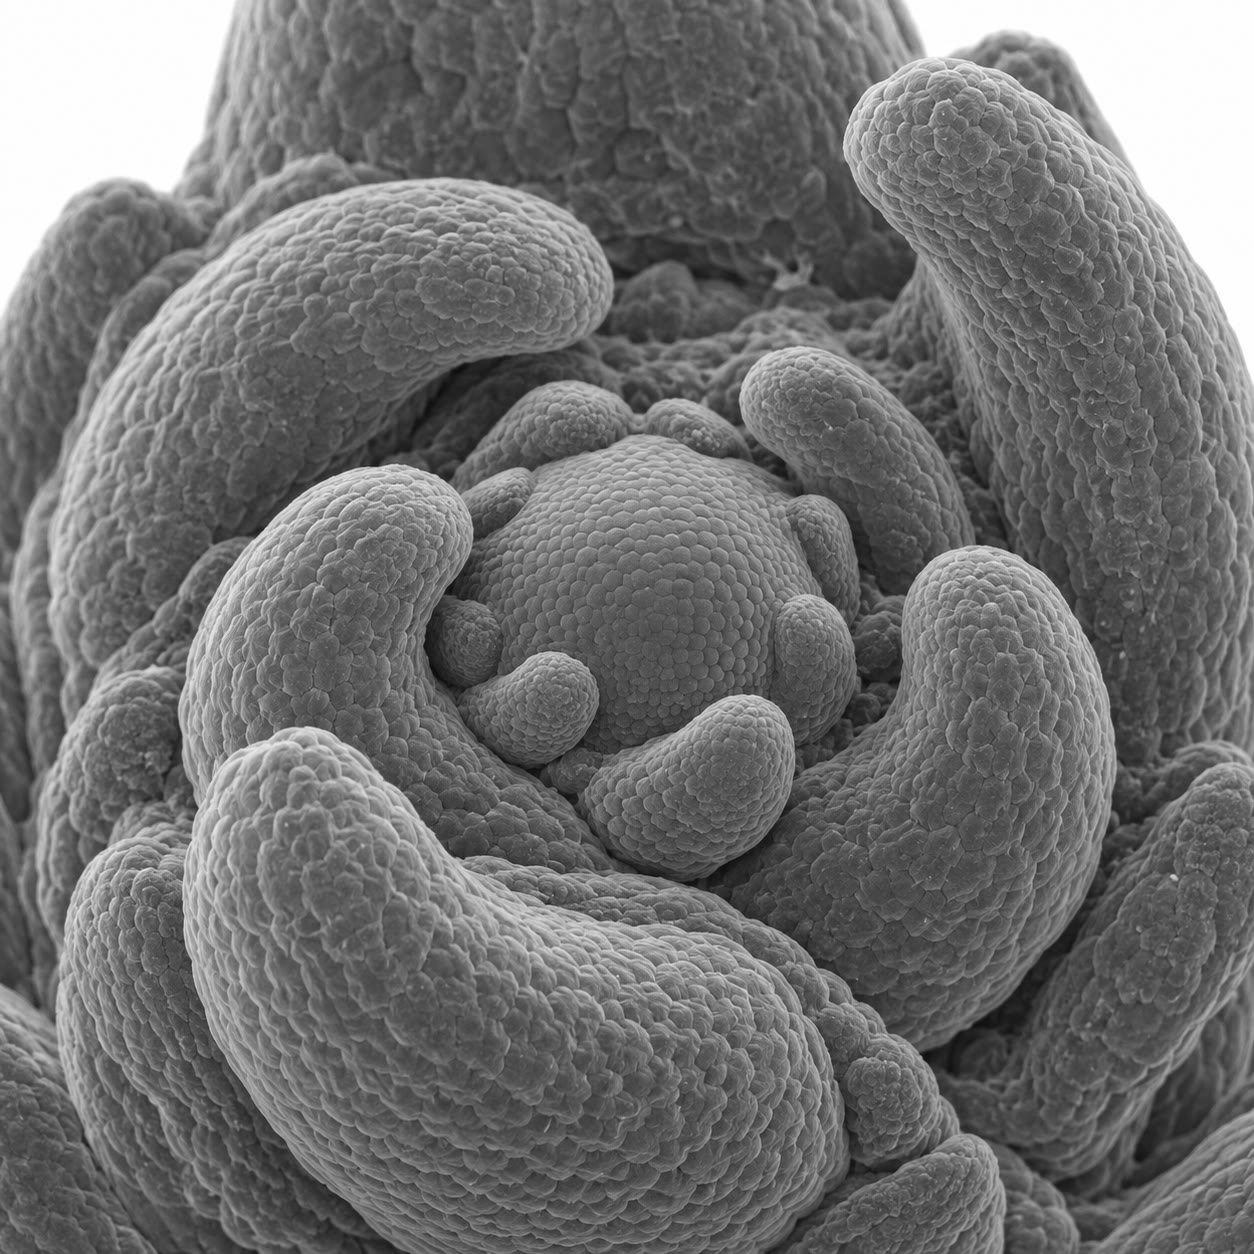
\includegraphics[width=0.44\linewidth]{images/book4/ai/b4-13-shoot-apex-sem.jpg}

{\small Een scheuttop onder de rasterelektronenmicroscoop: de gladde koepel
van het \omterm{def:b2:plant-meristems:meristem}{meristeem} en de spiraal van bladprimordia eromheen, elk nieuw
primordium in de breedste opening geplaatst.}
\end{omfigure}

\begin{proposition}[De stamcellen behouden: een terugkoppelingslus]\label{prop:b2:plant-meristems:wus}
\index{WUSCHEL}\index{CLAVATA}\index{negatieve terugkoppeling!meristeem}
De grootte van de stamcelvoorraad wordt constant gehouden door een lus
tussen twee genen. Cellen net onder de centrale zone brengen de
\omterm{prop:b2:cell-differentiation:transcriptional}{transcriptiefactor} \emph{WUSCHEL} (WUS) tot expressie, waarvan het product
naar de bovenliggende cellen beweegt en ze als stamcellen behoudt; de
stamcellen scheiden op hun beurt een klein peptide af, \emph{CLAVATA3}
(CLV3), dat naar beneden diffundeert, een receptorkinase (CLV1) in de cellen
die WUS tot expressie brengen bindt en WUS onderdrukt. Meer stamcellen
betekent meer CLV3, minder WUS, minder stamcellen; minder stamcellen betekent
minder CLV3, meer WUS, meer stamcellen. De voorraad is zo een geregelde
grootheid, zoals de gonadotrofinen van \cref{ch:b2:reproductive-hormones},
en dezelfde logica --- een signaal uit de geregelde populatie dat de factor
onderdrukt die haar maakt --- houdt ook het wortelmeristeem in stand.
\end{proposition}
\begin{proof}[Bewijsmateriaal]
\emph{clavata}-mutanten van Arabidopsis (Clark, Meyerowitz, jaren 1990)
hebben meristemen die opzwellen tot vele malen de normale grootte, met extra
bladeren, extra bloemorganen en gefascieerde (afgeplatte, lintvormige)
stengels: de rem is weg. \emph{wuschel}-mutanten maken een \omterm{def:b2:plant-meristems:meristem}{meristeem} dat na
enkele bladeren stopt en daarna nieuwe vormt, die elk op hun beurt stoppen:
het gaspedaal is weg. In de dubbelmutant overheerst het
\emph{wuschel}-fenotype, wat WUS stroomafwaarts van CLV plaatst; en
CLV3-peptide dat op een wildtype scheuttop wordt aangebracht, onderdrukt
WUS binnen enkele uren.
\end{proof}

\begin{proposition}[De worteltop]\label{prop:b2:plant-meristems:ram}
\index{wortelmutsje}\index{rustend centrum}\index{strekkingszone}\index{wortelhaar}
Een wortel groeit vanuit een \omterm{def:b2:plant-meristems:meristem}{meristeem} dat beschut ligt achter een
\emph{wortelmutsje}, waarvan de cellen worden afgeschuurd terwijl de top
door de grond dringt, en dat een smerend slijm afscheidt en de
zwaartekracht waarneemt (zetmeelkorrels die in zijn cellen neerslaan). In
het midden van het \omterm{def:b2:plant-meristems:meristem}{meristeem} deelt een \emph{\omterm{prop:b2:plant-meristems:ram}{rustend centrum}} van enkele
honderden cellen zich maar zelden; het houdt de omringende initialen --- van
het mutsje, de epidermis, de schors en de centrale cilinder --- als
stamcellen in stand, zoals WUS die van de scheut. Achter het \omterm{def:b2:plant-meristems:meristem}{meristeem} komt
de \emph{strekkingszone}, enkele millimeters waarin cellen tien- tot
twintigmaal langer worden en de top vooruitdrijven; dan de
\emph{differentiatiezone}, waar de epidermis \emph{wortelharen} vormt en
xyleem en floëem rijpen. Zijwortels ontstaan niet aan de top, maar uit de
pericykel, diep in de rijpe wortel, tegenover de xyleempolen, en dringen
naar buiten door de schors. Auxine, gemaakt in de scheut en naar beneden
gevoerd, hoopt zich in de top op en organiseert de hele opbouw; het
rustende centrum ligt op het maximum ervan.
\end{proposition}

\begin{omfigure}
\begin{tikzpicture}[every node/.style={font=\scriptsize}]
  % root outline
  \draw[thick, fill=omExo!10] (-1.0,4.5) -- (-1.0,0.6) .. controls (-1.0,-0.4) and (1.0,-0.4) .. (1.0,0.6) -- (1.0,4.5);
  % root cap
  \draw[thick, fill=omExo!45] (-0.9,0.8) .. controls (-1.1,-0.1) and (1.1,-0.1) .. (0.9,0.8) .. controls (0.5,0.4) and (-0.5,0.4) .. (-0.9,0.8);
  % meristem
  \fill[omThm!25] (-0.85,0.8) rectangle (0.85,1.7);
  \fill[omThm!70] (0,0.95) ellipse (0.25 and 0.12);
  % elongation zone
  \fill[omProp!20] (-0.85,1.7) rectangle (0.85,3.0);
  % differentiation zone with root hairs and vascular strand
  \fill[omDef!15] (-0.85,3.0) rectangle (0.85,4.5);
  \fill[omDef!50] (-0.15,3.0) rectangle (0.15,4.5);
  \foreach \y in {3.2,3.5,3.8,4.1,4.4} { \draw[omDef!80!black] (1.0,\y) -- (1.7,\y+0.1); \draw[omDef!80!black] (-1.0,\y) -- (-1.7,\y+0.1); }
  % lateral root primordium
  \draw[thick, fill=omThm!30] (0.15,4.0) .. controls (0.5,3.9) and (0.8,4.1) .. (0.9,4.3) .. controls (0.7,4.35) and (0.4,4.3) .. (0.15,4.3);
  % labels
  \draw (0.5,0.4) -- (2.2,0.2) node[right] {wortelmutsje};
  \draw (0.25,0.95) -- (2.2,0.9) node[right] {rustend centrum};
  \draw (0.85,1.4) -- (2.2,1.5) node[right] {meristeem (deling)};
  \draw (0.85,2.4) -- (2.2,2.3) node[right, align=left] {strekkingszone:\\cellen worden $10\times$ langer};
  \draw (1.5,3.6) -- (2.2,3.4) node[right] {wortelharen};
  \draw (0.0,4.2) -- (2.2,4.2) node[right] {centrale cilinder};
  \draw (0.7,4.3) -- (2.2,4.9) node[right, align=left] {primordium van een zijwortel\\(uit de pericykel)};
  \draw[->, thick] (-2.4,4.5) -- (-2.4,0.6); \node[left, rotate=90, anchor=south] at (-2.5,2.5) {auxine stroomt naar de top};
\end{tikzpicture}

{\small De worteltop: mutsje, \omterm{def:b2:plant-meristems:meristem}{meristeem} met zijn rustende centrum,
strekkingszone, en de differentiatiezone met wortelharen en rijpe vaten.
Zijwortels beginnen diep binnenin, vanuit de pericykel.}
\end{omfigure}

\begin{omfigure}
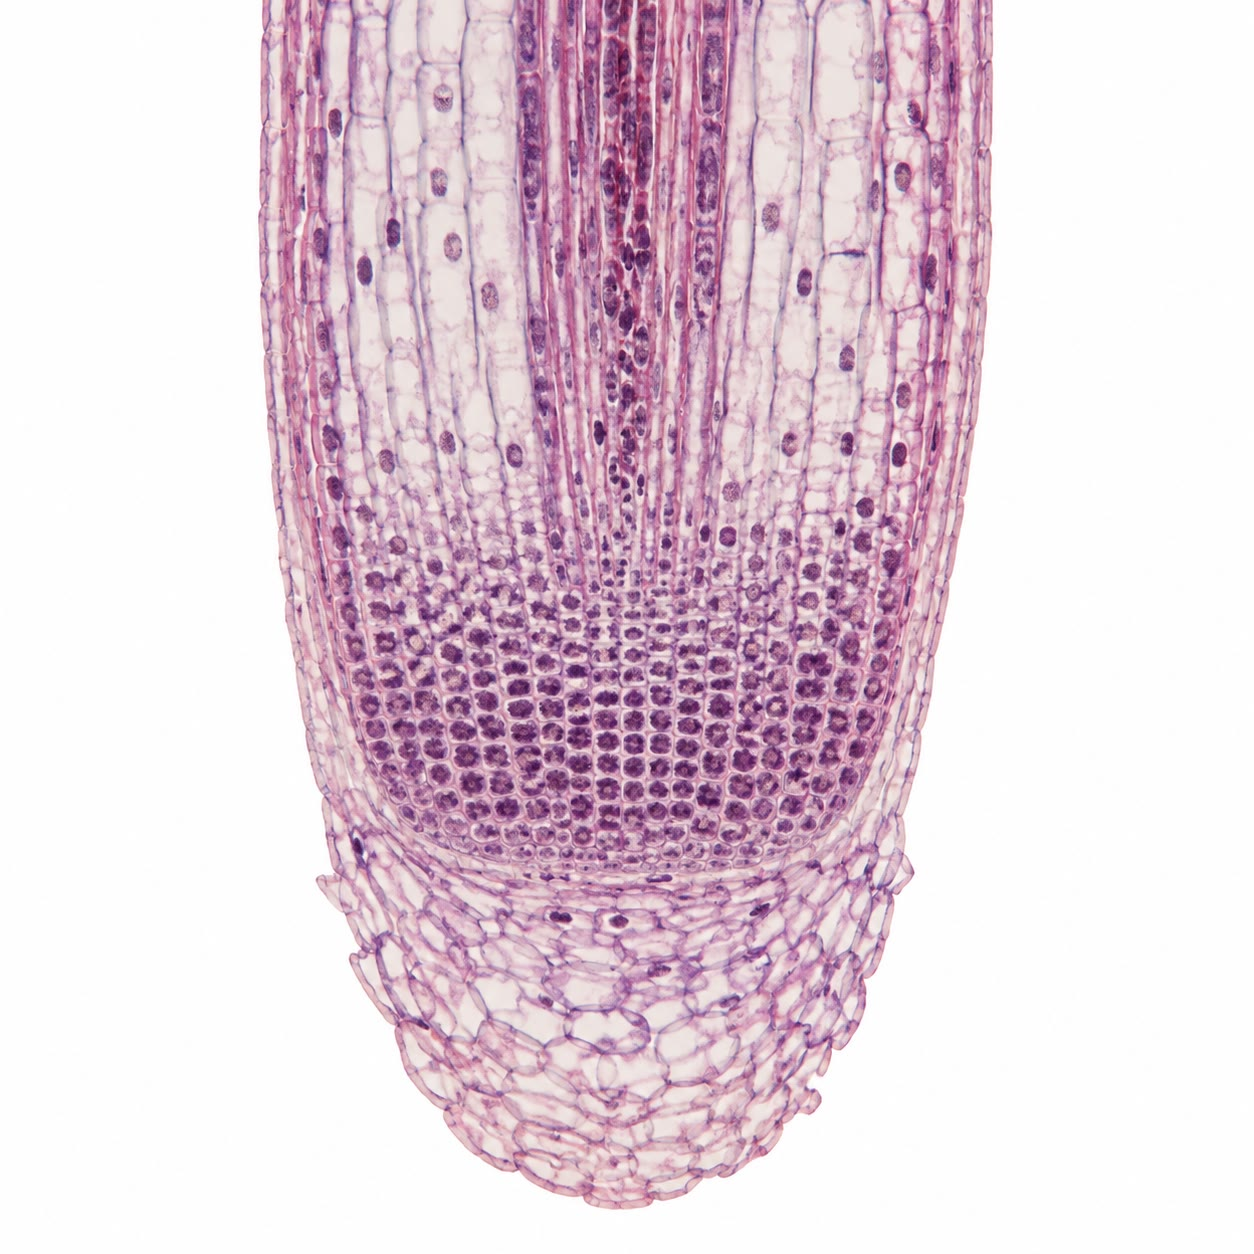
\includegraphics[width=0.42\linewidth]{images/book4/ai/b4-13-root-tip.jpg}

{\small Een worteltop in lengtedoorsnede: de losse cellen van het mutsje,
het dichte \omterm{def:b2:plant-meristems:meristem}{meristeem} met zijn donkere kernen, en de zich strekkende cellen
erboven.}
\end{omfigure}

\section{Hoe een plantencel groeit}

\begin{theorem}[De vergelijking van Lockhart]\label{thm:b2:plant-meristems:lockhart}
\index{turgor}\index{celwand!rekbaarheid}\index{vergelijking van Lockhart}
Een plantencel groeit door haar wand op te rekken onder de druk van haar
eigen inhoud. De wand geeft alleen onomkeerbaar mee boven een drempel van de
turgor $Y$, en dan met een snelheid die evenredig is met het overschot: de
relatieve groeisnelheid van een cel met lengte $L$ is
\[
\frac{1}{L}\frac{\mathrm{d}L}{\mathrm{d}t} = \phi\,(P - Y) \quad (P > Y),
\]
waarin $P$ de turgordruk is en $\phi$ de \emph{rekbaarheid} van de wand. De
groei wordt dus van twee kanten gestuurd: door water, dat $P$ bepaalt (een
verwelkende cel houdt op met groeien), en door de wand, die $\phi$ en $Y$
bepaalt --- en het is op de wand dat hormonen inwerken. Auxine laat cellen
protonen in de wand pompen; het zuur activeert \emph{expansinen}, eiwitten
die de bindingen tussen cellulosefibrillen en de matrix losmaken, waardoor
$\phi$ binnen enkele minuten stijgt en $Y$ daalt (\emph{zuurgroei}). Met
$\phi =
\qty{0.1}{h^{-1}.MPa^{-1}}$, $Y = \qty{0.3}{MPa}$ en $P =
\qty{0.6}{MPa}$ wordt een cel \qty{3}{\%} per uur langer en verdubbelt ze in
een dag; in de strekkingszone van een wortel, waar de snelheden meermaals
hoger zijn, wordt een cel in enkele uren tien keer zo lang.
\end{theorem}
\begin{proof}
De wand is een viscoplastisch materiaal: onder de zwichtspanning vervormt
hij elastisch en herstelt hij zich, erboven vloeit hij met een snelheid die
evenredig is met de overmaat aan spanning. De spanning in de wand is
evenredig met de turgordruk (voor een cilinder met straal $r$ en wanddikte
$w$ is de ringspanning $Pr/w$), zodat de plastische rekkingssnelheid
evenredig is met $P - Y$, met een constante $\phi$ die de geometrie en de
materiaaleigenschappen van de wand omvat. De rekkingssnelheid is per
definitie $(1/L)\,\mathrm{d}L/\mathrm{d}t$. Numeriek is
$0.1\times(0.6 - 0.3) = \qty{0.03}{h^{-1}}$, en $L$ verdubbelt wanneer
$0.03\,t = \ln 2$, $t = \qty{23}{h}$.
\end{proof}

\begin{omfigure}
\begin{tikzpicture}
\begin{axis}[
  width=0.7\linewidth, height=5.4cm,
  axis x line=bottom, axis y line=left,
  xmin=0, xmax=1.0, ymin=0, ymax=0.09,
  xlabel={turgordruk $P$ (\unit{MPa})}, ylabel={relatieve groeisnelheid (\unit{h^{-1}})},
  xlabel style={font=\small, at={(axis description cs:0.5,-0.13)}, anchor=north},
  ylabel style={font=\small},
  tick label style={font=\small}, xtick={0,0.3,0.6,0.9}, ytick={0,0.03,0.06,0.09},
  yticklabels={0,0.03,0.06,0.09}, scaled y ticks=false,
  legend style={font=\scriptsize, at={(0.03,0.97)}, anchor=north west, draw=none},
  clip=false,
]
\addplot[very thick, omDef, domain=0:0.3, samples=2, forget plot] {0};
\addplot[very thick, omDef, domain=0.3:1.0, samples=2] {0.1*(x-0.3)};
\addlegendentry{$\phi = 0.1$, $Y = 0.3$}
\addplot[very thick, omThm, domain=0:0.2, samples=2, forget plot] {0};
\addplot[very thick, omThm, domain=0.2:0.65, samples=2] {0.2*(x-0.2)};
\addlegendentry{met auxine: $\phi = 0.2$, $Y = 0.2$}
\draw[dashed, gray] (axis cs:0.6,0) -- (axis cs:0.6,0.03); \node[font=\scriptsize, anchor=west] at (axis cs:0.61,0.015) {typische $P$};
\end{axis}
\end{tikzpicture}

{\small De wet van Lockhart: geen groei onder de zwichtturgor, daarna een
snelheid die evenredig is met het overschot. Auxine verlaagt, door de wand
los te maken, de drempel en maakt de lijn steiler, zodat de cel bij dezelfde
turgor meermaals sneller groeit.}
\end{omfigure}

\begin{example}[Waar het water vandaan komt]\label{ex:b2:plant-meristems:water}
Terwijl de wand meegeeft, zou de turgor dalen en de groei stoppen, als er
niet voldoende water binnenkwam om bij te blijven: de groeiende cel is een
lek dat zichzelf bijvult. Het water komt uit het xyleem, langs een kleine
gradiënt in waterpotentiaal, en de snelheid waarmee het binnenkomt, wordt
bepaald door de hydraulische geleidbaarheid van het membraan; de groei is
's nachts het snelst, wanneer de transpiratie laag en de turgor hoog is,
en een maïsblad kan tussen schemering en dageraad \qty{10}{cm} langer
worden. Bij droogte maken de cellen opgeloste stoffen (\emph{osmotische
aanpassing}) om $P$ boven $Y$ te houden, en als dat mislukt, houdt het blad
dagen voordat het verwelkt al op met groeien.
\end{example}

\section{Hormonen en de vorm van de scheut}

\begin{proposition}[Auxine en apicale dominantie]\label{prop:b2:plant-meristems:apical}
\index{auxine}\index{apicale dominantie}\index{polair auxinetransport}\index{cytokinine}
\emph{Auxine} (indool-3-azijnzuur) wordt gemaakt in de scheuttop en jonge
bladeren en door de stengel naar beneden gevoerd, van cel tot cel, met
ongeveer \qty{1}{cm/h}, door dragereiwitten (PIN) in het onderste uiteinde
van elke cel --- een \emph{polair transport} dat de plant een as van boven
naar onder geeft. De stroom auxine die uit de top neerdaalt, houdt de
okselknoppen eronder in rust (\emph{\omterm{prop:b2:plant-meristems:apical}{apicale dominantie}}), deels door te
verhinderen dat ze hun eigen auxine naar de stengel afvoeren, deels door
strigolactonen te induceren en cytokinine te onderdrukken. Snijd de top
weg, en de knoppen die het dichtst bij de snede zitten, lopen binnen enkele
dagen uit, wat een struikvormige plant oplevert --- en daarvan maken snoeien
en toppen gebruik. \emph{Cytokininen}, gemaakt in de worteltoppen en via
het xyleem omhoog gevoerd, bevorderen het uitlopen van knoppen en de
celdeling; \emph{gibberellinen} verlengen de internodia (dwergerwten en de
halfdwergtarwe van de Groene Revolutie schieten tekort in het maken of
waarnemen ervan); abscisinezuur en ethyleen remmen de groei bij stress. De
vorm van de scheut --- hoog of struikvormig, rechtop of uitgespreid --- is
een onderhandeling tussen deze signalen, en het evenwicht tussen wortel en
scheut wordt bepaald door de auxine die naar beneden gaat tegenover de
cytokinine die omhoogkomt.
\end{proposition}
\begin{proof}[Bewijsmateriaal]
Thimann en Skoog (1934) sneden de top van bonenplanten weg: de zijknoppen
groeiden uit. Een agarblokje met auxine op de afgesneden stomp hield ze in
rust, zoals de top had gedaan; gewone agar niet. Went (1928) had auxine al
gemeten aan de hand van de kromming die het veroorzaakte in onthoofde
coleoptielen van haver wanneer het op één kant van de stomp werd
geplaatst --- de eerste biotoets van een plantenhormoon, en de oorsprong
van de naam, naar het Griekse woord voor ``groeien''. De polariteit van het
transport werd aangetoond door auxineagar op één uiteinde van een
stengelsegment te plaatsen en het in een ontvangstblokje aan het andere
uiteinde terug te vinden alleen wanneer het segment met de top naar boven
lag, hoe het segment ook in het zwaarteveld werd gedraaid.
\end{proof}

\begin{omfigure}
\begin{tikzpicture}[every node/.style={font=\scriptsize}, >=stealth]
  \foreach \x/\lab/\apex/\aux in {0/{intact: top aanwezig,\\knoppen in rust}/1/0, 4.2/{top verwijderd:\\knoppen lopen uit}/0/0, 8.4/{top verwijderd + auxine\\op de stomp: in rust}/0/1} {
    \begin{scope}[xshift=\x cm]
      \draw[very thick, omExo!70!black] (0,0) -- (0,3.4);
      \foreach \y in {0.8,1.6,2.4} { \draw[thick, omExo!70!black] (0,\y) -- (-0.8,\y+0.4); \draw[thick, omExo!70!black] (0,\y+0.4) -- (0.8,\y+0.8); }
      \ifnum\apex=1 \draw[thick, fill=omThm!40] (0,3.5) ellipse (0.25 and 0.3); \draw[->, thick, omThm] (0.35,3.2) -- (0.35,1.0); \node[omThm, right] at (0.4,2.1) {auxine}; \fi
      \ifnum\apex=0 \draw[thick] (-0.3,3.4) -- (0.3,3.4); \fi
      \ifnum\aux=1 \draw[thick, fill=omThm!40] (-0.25,3.4) rectangle (0.25,3.75); \node[omThm, right] at (0.3,3.6) {auxineagar}; \draw[->, thick, omThm] (0.35,3.2) -- (0.35,1.0); \fi
      \ifnum\apex=1 \foreach \y in {0.8,1.6,2.4} \fill[gray!60] (-0.12,\y+0.1) circle (0.08); \fi
      \ifnum\aux=1 \foreach \y in {0.8,1.6,2.4} \fill[gray!60] (-0.12,\y+0.1) circle (0.08); \fi
      \ifnum\apex=0 \ifnum\aux=0 \foreach \y in {0.8,1.6,2.4} { \draw[thick, omExo!70!black] (-0.1,\y+0.1) -- (-0.7,\y+0.9); \draw[thick, omExo!70!black] (-0.7,\y+0.9) -- (-1.0,\y+1.1); \draw[thick, omExo!70!black] (-0.7,\y+0.9) -- (-0.75,\y+1.25); } \fi\fi
      \node[below, align=center] at (0,-0.3) {\lab};
    \end{scope}
  }
\end{tikzpicture}

{\small \omterm{prop:b2:plant-meristems:apical}{Apicale dominantie}, het experiment van Thimann en Skoog. De top houdt
de okselknoppen in rust; hem verwijderen laat ze los; auxine op de
afgesneden stomp vervangt de top.}
\end{omfigure}

\begin{example}[Snel signaal, traag molecuul]\label{ex:b2:plant-meristems:transport}
Polair transport verplaatst auxine \qty{1}{cm} in een uur; diffusie alleen
zou voor dezelfde centimeter $t = x^2/2D = 10^{-4}/(2\times
10^{-9}) = \qty{5e4}{s}$ nodig hebben --- veertien uur --- en voor de
tien centimeter tot een lagere knop zestig dagen. Het pompen en doorgeven
door de PIN-dragers maakt een hormonaal signaal bruikbaar over de lengte
van een plant; dezelfde dragers, naar de beschaduwde kant van een stengel
verplaatst, buigen hem naar het licht toe (\cref{ch:b2:plant-plasticity}).
\end{example}

\section{Secundaire groei: hout en schors}

\begin{definition}[Het vaatcambium en hout]\label{def:b2:plant-meristems:wood}
\index{vaatcambium}\index{hout}\index{jaarring}\index{schors}\index{periderm}
In een houtige stengel worden de strengen primair xyleem en floëem in het
eerste jaar verbonden tot een doorlopende cilinder van delende cellen, het
\emph{vaatcambium}. Zijn cellen delen zich tangentiaal en voegen
\emph{secundair xyleem} --- \emph{hout} --- aan de binnenkant toe en
\emph{secundair floëem} aan de buitenkant, zodat het \omterm{def:b2:plant-meristems:meristem}{cambium} naar buiten
opschuift terwijl de stam dikker wordt, met af en toe een radiale deling om
de ring te verbreden. In seizoensklimaten heeft het hout dat in het voorjaar
wordt aangelegd wijde, dunwandige vaten (\emph{vroeghout}) en dat van de
zomer nauwe, dikwandige (\emph{laathout}), zodat elk jaar een zichtbare
\emph{jaarring} achterlaat; de ringen leggen de leeftijd van de boom vast
en, in hun breedte, het klimaat van elk jaar (dendrochronologie). Alleen de
buitenste ringen, het \emph{spinthout}, geleiden; de binnenste, het
\emph{kernhout}, zijn dood, verstopt en gedonkerd door harsen en tannines,
en dienen als skelet van de boom. Buiten het floëem maakt een tweede
lateraal \omterm{def:b2:plant-meristems:meristem}{meristeem}, het \emph{kurkcambium}, het \emph{periderm} --- lagen
kurkcellen, dood en met suberine waterdicht gemaakt --- dat samen met het
oude floëem de \emph{schors} vormt. Een stam is dus een dunne levende schil
van \omterm{def:b2:plant-meristems:meristem}{cambium}, spinthout en floëem rond een dode kern, onder een dode huid.
\end{definition}

\begin{omfigure}
\begin{tikzpicture}[every node/.style={font=\scriptsize}]
  \fill[omExo!60] (0,0) circle (3.0);
  \fill[omDef!20] (0,0) circle (2.75);
  \fill[omDef!35] (0,0) circle (2.2);
  \foreach \r in {0.4,0.7,1.0,1.3,1.6,1.9,2.2} \draw[omDef!80!black, thin] (0,0) circle (\r);
  \fill[omExo!80!black] (0,0) circle (1.3);
  \foreach \r in {0.4,0.7,1.0} \draw[omExo!40, thin] (0,0) circle (\r);
  \draw[very thick, omThm] (0,0) circle (2.5);
  \draw (2.9,0.6) -- (3.9,1.6) node[right, align=left] {schors: kurk (periderm)\\en oud floëem};
  \draw (2.62,0.0) -- (3.9,0.6) node[right] {secundair floëem, levend};
  \draw (2.5,-0.4) -- (3.9,-0.4) node[right] {vaatcambium (rood)};
  \draw (1.9,-1.1) -- (3.9,-1.4) node[right, align=left] {spinthout: recente ringen,\\geleidend};
  \draw (0.5,-0.9) -- (3.9,-2.4) node[right, align=left] {kernhout: oude ringen,\\dood, verstopt};
  \draw (-1.7,1.5) -- (-3.6,2.4) node[left, align=right] {één jaarring:\\licht vroeghout,\\donker laathout};
\end{tikzpicture}

{\small Een stam in dwarsdoorsnede. Het \omterm{def:b2:plant-meristems:meristem}{cambium} (rood) voegt elk jaar \omterm{def:b2:plant-meristems:wood}{hout}
naar binnen en floëem naar buiten toe; de recente ringen geleiden, de oude
vormen het dode kernhout; kurk en oud floëem vormen de schors.}
\end{omfigure}

\begin{theorem}[Waarom een oude boom meer hout aanmaakt]\label{thm:b2:plant-meristems:rings}
Een stam met straal $r$ en hoogte $h$ waarvan het \omterm{def:b2:plant-meristems:meristem}{cambium} elk jaar een ring
met dikte $\Delta r$ toevoegt, wint per jaar een houtvolume
\[
\Delta V \approx 2\pi r\,h\,\Delta r
\]
zodat bij een constante ringbreedte de jaarlijkse aanwas evenredig groeit met
de straal, en een boom met een straal van \qty{50}{cm} maakt tien keer zoveel
\omterm{def:b2:plant-meristems:wood}{hout} aan als een boom met \qty{5}{cm}, hoewel zijn ringen niet breder zijn.
Een stam met een straal van \qty{25}{cm} en een hoogte van \qty{10}{m} die
\qty{4}{mm} per jaar aangroeit, wint \qty{0.063}{m^3}, ongeveer \qty{30}{kg}
droog \omterm{def:b2:plant-meristems:wood}{hout} --- \qty{15}{kg} koolstof, in één seizoen door de kroon uit de
lucht gehaald.
\end{theorem}
\begin{proof}
Het toegevoegde \omterm{def:b2:plant-meristems:wood}{hout} is een cilindrische schil met omtrek $2\pi r$, dikte
$\Delta r$ en hoogte $h$; het volume is $2\pi r h\Delta r$ in eerste orde in
$\Delta r$ (exact $\pi h[(r + \Delta r)^2 - r^2]
= \pi h(2r\Delta r + \Delta r^2)$). Met $r = 0.25$, $h = 10$,
$\Delta r = 0.004$: $2\pi\times 0.25\times 10\times 0.004 =
\qty{0.063}{m^3}$; bij \qty{500}{kg/m^3} droog \qty{31}{kg}, waarvan de
helft koolstof.
\end{proof}

\begin{omfigure}
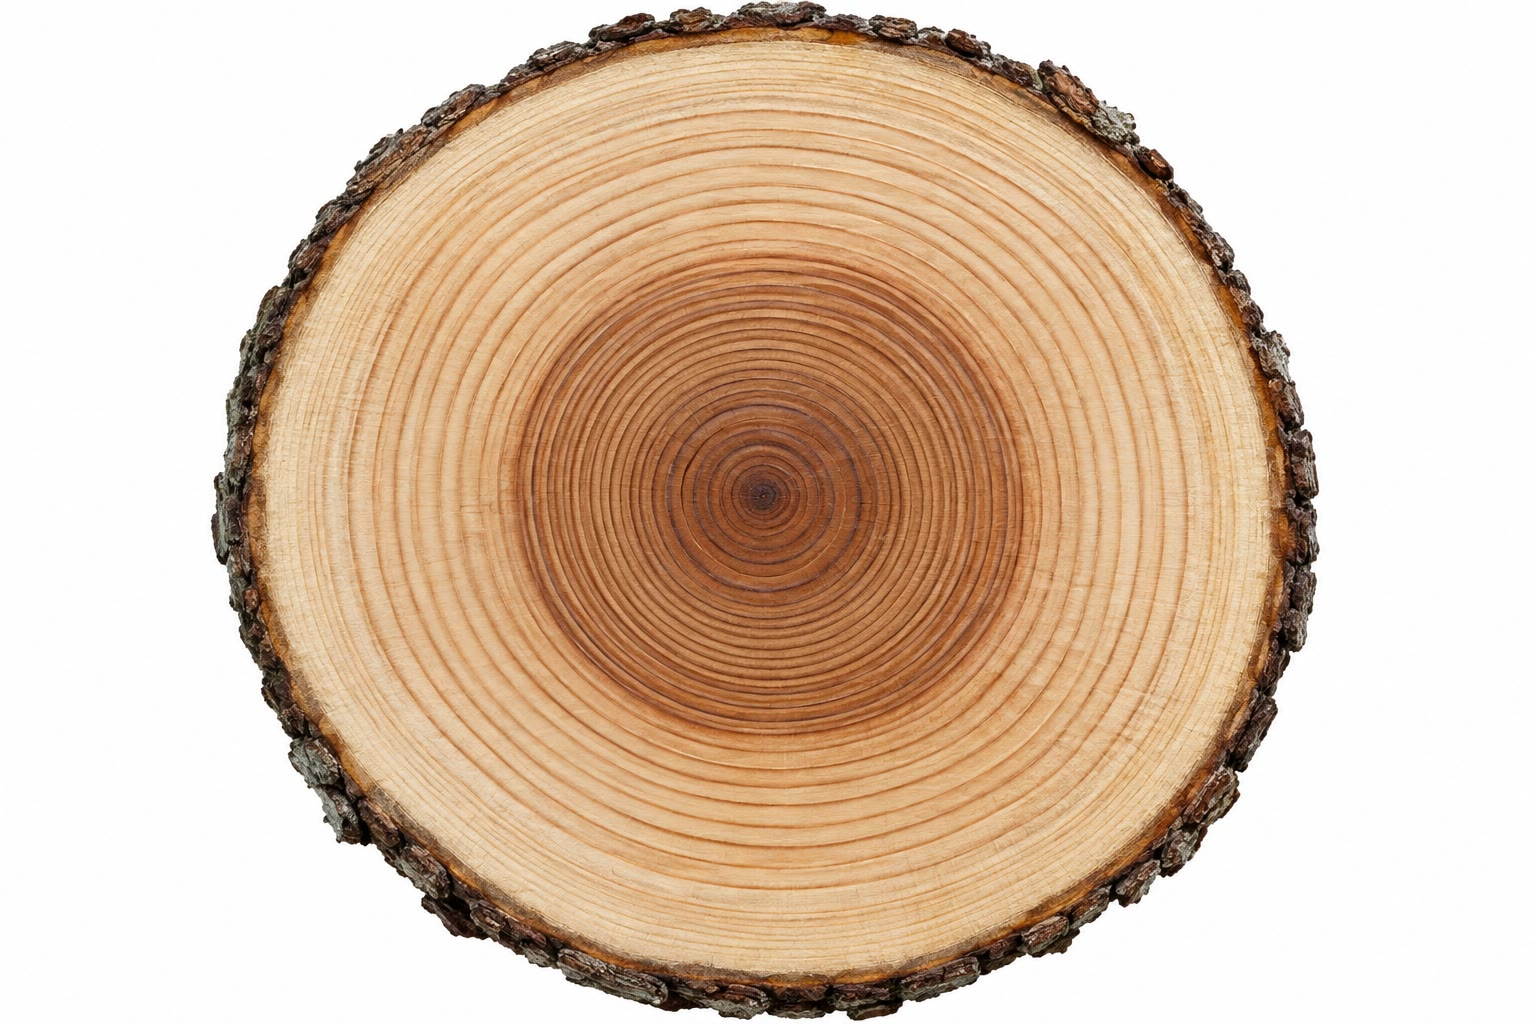
\includegraphics[width=0.5\linewidth]{images/book4/ai/b4-13-wood-rings.jpg}

{\small Een dennenstam in dwarsdoorsnede: de \omterm{def:b2:plant-meristems:wood}{jaarringen}, elk een lichte
band vroeghout en een donkere band laathout, het donkerdere kernhout, en de
schors.}
\end{omfigure}

\section{Opgaven}

\begin{exercise}[$\star$]\label{exo:b2:plant-meristems:1}
Definieer \omterm{def:b2:plant-meristems:meristem}{meristeem}, en noem de vier meristemen van een houtige plant met
wat elk ervan voortbrengt.
\end{exercise}

\begin{exercise}[$\star$]\label{exo:b2:plant-meristems:2}
Noem de zones van een worteltop van het mutsje naar boven, met wat er in
elke zone met een cel gebeurt. Waar komen zijwortels vandaan?
\end{exercise}

\begin{exercise}[$\star$]\label{exo:b2:plant-meristems:3}
Beschrijf het experiment van Thimann en Skoog, de controle ervan en de
conclusie.
\end{exercise}

\begin{exercise}[$\star$]\label{exo:b2:plant-meristems:4}
Een doorsnede van een stam toont 60 ringen, waarvan de buitenste 15 licht en
de rest donker. Geef de leeftijd van de boom, de leeftijd van zijn
spinthout, en zeg welk deel van de stam leeft.
\end{exercise}

\begin{exercise}[$\star\star$]\label{exo:b2:plant-meristems:5}
Bereken met $\phi = \qty{0.1}{h^{-1}.MPa^{-1}}$ en $Y = \qty{0.3}{MPa}$
de relatieve groeisnelheid bij $P = 0.4$, $0.6$ en \qty{0.8}{MPa}, en de
verdubbelingstijd bij elke waarde. Een droogte verlaagt $P$ tot
\qty{0.25}{MPa}: wat gebeurt er?
\end{exercise}

\begin{exercise}[$\star\star$]\label{exo:b2:plant-meristems:6}
Opeenvolgende bladeren ontstaan onder \qty{137.5}{\degree} van elkaar.
Bereken de hoekposities van blad 1 tot 8 (modulo
\qty{360}{\degree}) en toon aan dat geen twee van de eerste acht binnen
\qty{20}{\degree} van elkaar liggen. Waarom doet dit er voor de plant toe?
\end{exercise}

\begin{exercise}[$\star\star$]\label{exo:b2:plant-meristems:7}
Een boom van \qty{12}{m} hoog legt ringen van \qty{3}{mm} aan. Bereken het
\omterm{def:b2:plant-meristems:wood}{hout} dat wordt toegevoegd in het jaar waarin zijn straal \qty{5}{cm} is en
in het jaar waarin die \qty{40}{cm} is, en de bijbehorende koolstof (droge
dichtheid \qty{500}{kg/m^3}, voor de helft koolstof).
\end{exercise}

\begin{exercise}[$\star\star$]\label{exo:b2:plant-meristems:8}
Voorspel de \omterm{def:b2:meiosis-heredity:vocabulary}{fenotypen} van een \emph{clv3}-mutant, een \emph{wus}-mutant en de
dubbelmutant, en leg uit hoe de dubbelmutant de volgorde van de twee genen
in de lus vastlegt.
\end{exercise}

\begin{exercise}[$\star\star$]\label{exo:b2:plant-meristems:9}
Auxine wordt met \qty{1}{cm/h} getransporteerd; de diffusiecoëfficiënt in
weefsel is \qty{1e-9}{m^2/s}. Hoelang doet het signaal erover om een knop
\qty{20}{cm} onder de top te bereiken door transport, en door diffusie
($t = x^2/2D$)? Wat levert polair transport de plant op?
\end{exercise}

\begin{exercise}[$\star\star\star$]\label{exo:b2:plant-meristems:10}
Een maïswortel groeit \qty{3}{cm} per dag. Meristeemcellen zijn
\qty{20}{\micro m} lang en worden tien keer langer voordat ze rijpen; elke
celrij heeft ongeveer \num{100} delende cellen. Hoeveel cellen moet het
\omterm{def:b2:plant-meristems:meristem}{meristeem} van elke rij per dag maken, en welke celcyclusduur volgt daaruit?
\end{exercise}

\begin{exercise}[$\star\star\star$]\label{exo:b2:plant-meristems:11}
De halfdwergtarwes uit de jaren 1960 dragen \omterm{def:b2:genome-diversification:mutation}{mutaties} die de plant
ongevoelig maken voor gibberelline. Leg uit waarom ze kort zijn, waarom een
korte plant bij zware bemesting meer graan kan opbrengen, en waarom dezelfde
\omterm{def:b2:genome-diversification:mutation}{mutatie} bij een wilde plant een nadeel zou zijn.
\end{exercise}

\begin{exercise}[$\star\star\star$]\label{exo:b2:plant-meristems:12}
``Een dier wordt één keer gebouwd; een plant wordt haar hele leven
gebouwd.'' Bespreek de gevolgen van meristematische groei voor het vermogen
van een plant om op haar omgeving te reageren, schade te overleven en
millennia te leven --- en één nadeel van de strategie.
\end{exercise}

\section{Vraagstuk: een boom in getallen}

\begin{problem}[{Weekendvraagstuk --- een jonge boom een jaar lang gevolgd:
de bladeren die zijn top maakt, de groei van een internodium volgens de wet
van Lockhart, het hout dat zijn cambium aanlegt en de koolstof die dat
kost, en de reactie van zijn knoppen op snoeien, met als besluit de
bladeren per jaar, de groei van het internodium per uur en het hout van het
jaar}]
\label{pb:b2:plant-meristems:1}
Een jonge linde heeft \num{200} groeiende scheuttoppen; elke top legt tijdens
een seizoen van \num{150} dagen om de \num{3} dagen een blad aan, met
tussenhoeken van \qty{137.5}{\degree}. Een groeiend internodium is
\qty{2}{cm} lang, zijn cellen hebben $\phi = \qty{0.05}{h^{-1}.MPa^{-1}}$,
$Y =
\qty{0.35}{MPa}$; de turgor is overdag \qty{0.55}{MPa} en 's nachts
\qty{0.75}{MPa} (elk \qty{12}{h}). De stam is \qty{8}{m} hoog met een straal
van \qty{10}{cm}; het \omterm{def:b2:plant-meristems:meristem}{cambium} voegt \qty{5}{mm} per jaar toe; droog \omterm{def:b2:plant-meristems:wood}{hout}
weegt \qty{500}{kg/m^3} en bestaat voor de helft uit koolstof. De kroon draagt
\qty{80}{m^2} bladeren die netto \qty{4}{g} koolstof per vierkante meter per
dag vastleggen, gedurende \num{150} dagen.

\medskip
\noindent\textbf{Deel I --- Bladeren.}
\begin{enumerate}
  \item Hoeveel bladeren maakt één top in een seizoen? De hele boom?
  \item Bereken de hoekposities van blad 1 tot 5 op één scheut.
  \item Na hoeveel bladeren valt een blad binnen \qty{10}{\degree} van
        blad 1? (Probeer veelvouden van \qty{137.5}{\degree}.)
  \item Wat bereikt de gulden hoek voor de plant, en het transport van welk
        hormoon brengt hem voort?
  \item Als elk blad een oppervlakte van \qty{80}{cm^2} heeft, welke
        bladoppervlakte bouwt de boom dan in een seizoen? Vergelijk met de
        \qty{80}{m^2} die hij midden in de zomer draagt.
  \item De boom is bladverliezend. Welk deel van zijn bladoppervlak bouwt
        hij elk voorjaar opnieuw op, en waar komt de koolstof voor de eerste
        bladeren vandaan?
  \item Een \emph{clv3}-mutatie verdrievoudigt de grootte van elke top.
        Wat zou er veranderen in de antwoorden op vraag 1 en 5, en hoe zouden
        de scheuten eruitzien?
\end{enumerate}

\medskip
\noindent\textbf{Deel II --- Een internodium.}
\begin{enumerate}[resume]
  \item Bereken de relatieve groeisnelheid overdag en 's nachts.
  \item Bereken de lengte die in één dag en één nacht wordt toegevoegd,
        uitgaande van \qty{2}{cm}.
  \item Wat is de lengte van het internodium na vier zulke etmalen?
        (Behandel de groei als samengesteld, $L(t) = L_0 e^{rt}$ met de
        gemiddelde snelheid.)
  \item Een behandeling met gibberelline verlaagt $Y$ tot \qty{0.25}{MPa}.
        Bereken de snelheden overdag en 's nachts opnieuw.
  \item Een droogte houdt de turgor dag en nacht op \qty{0.4}{MPa}.
        Bereken de snelheid, en zeg wat osmotische aanpassing doet.
  \item Leg uit waarom de groei 's nachts groter is dan overdag, hoewel de
        fotosynthese overdag plaatsvindt.
\end{enumerate}

\medskip
\noindent\textbf{Deel III --- \omterm{def:b2:plant-meristems:wood}{Hout}.}
\begin{enumerate}[resume]
  \item Bereken het volume \omterm{def:b2:plant-meristems:wood}{hout} dat dit jaar is toegevoegd en de droge massa
        ervan.
  \item Bereken de koolstof daarin.
  \item Bereken de koolstof die de kroon over het seizoen heeft vastgelegd.
  \item Welk deel van de koolstof van de kroon ging naar stamhout? Noem
        drie andere bestemmingen.
  \item Wat zal de jaarlijkse houtaanwas over twintig jaar zijn, bij
        dezelfde ringbreedte? Waarom stijgt die?
  \item Twee ringen van de stam zijn half zo breed als hun buren. Geef twee
        mogelijke oorzaken en zeg hoe een dendrochronoloog ze uit elkaar zou
        houden.
\end{enumerate}

\medskip
\noindent\textbf{Deel IV --- Knoppen en snoeien.}
\begin{enumerate}[resume]
  \item De tuinier snoeit elke scheuttop terug. Voorspel de reactie van de
        okselknoppen en de vorm van de boom na een maand.
  \item Hoe zou een auxinepasta op elke snede de reactie veranderen?
  \item Een haag wordt zes keer per jaar geknipt. Leg met de \omterm{prop:b2:plant-meristems:apical}{apicale
        dominantie} uit waarom ze dicht wordt.
  \item Een tot een stobbe afgezette boom loopt uit met een dozijn scheuten.
        Waar komen ze vandaan, en waarom kan een plant het verlies van elke
        scheut overleven, terwijl een dier het verlies van zijn kop niet
        overleeft?
  \item Cytokinine uit de wortels neemt toe nadat de wortels water hebben
        gekregen. Voorspel het effect op het uitlopen van de knoppen.
  \item Formuleer het resultaat: bladeren per top en per boom per seizoen,
        de groeisnelheden van het internodium overdag en 's nachts, en het
        \omterm{def:b2:plant-meristems:wood}{hout} en de koolstof van het jaar.
\end{enumerate}
\end{problem}
